\chapter{Database Schema}
\label{ch:database-schema}

% Diagram first
\begin{figure}[H]
\centering
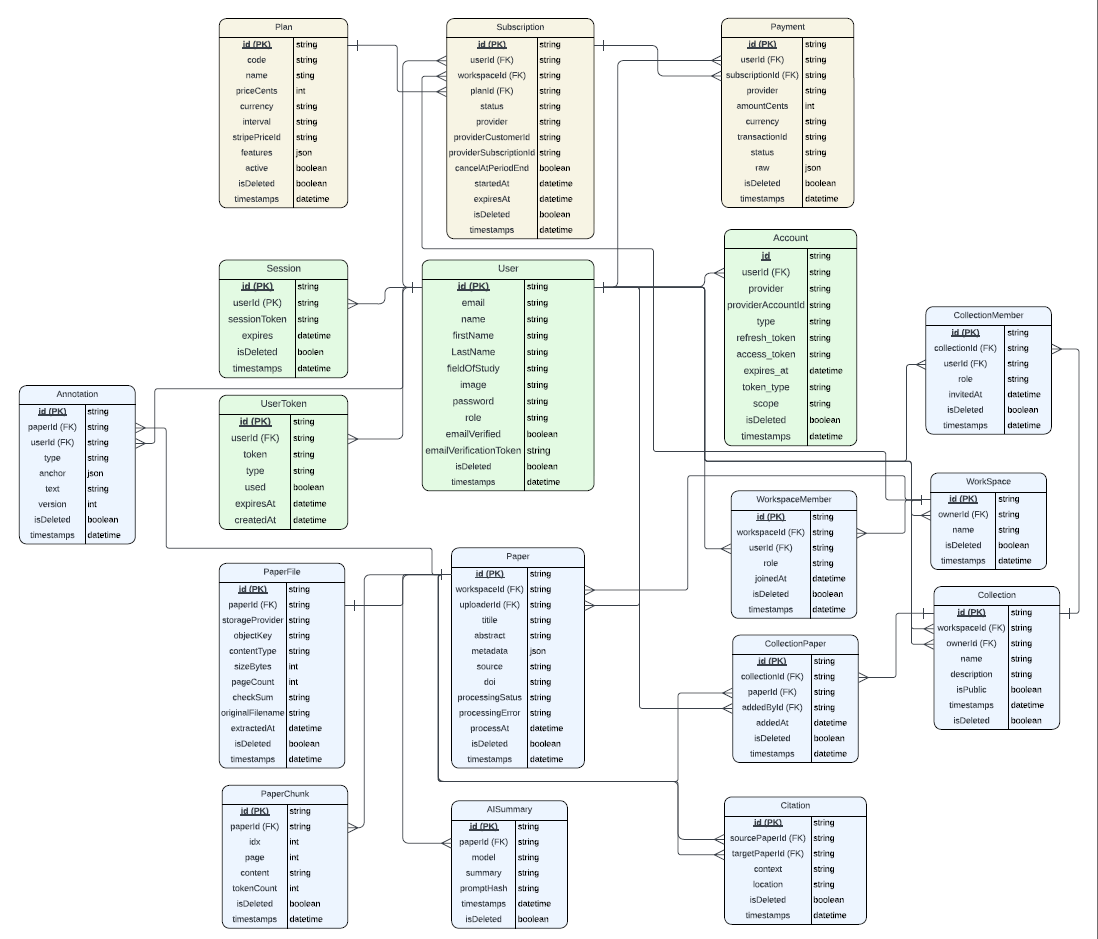
\includegraphics[width=0.95\textwidth]{images/diagrams/schema.png}
\caption{High-level database schema of ScholarFlow}
\label{fig:db-schema}
\end{figure}

% One-page key information
\section*{Key Information}
\begin{itemize}[leftmargin=*,topsep=3pt,itemsep=2pt]
  \item \textbf{Core Entities}: User, Paper, Collection, Workspace, WorkspaceMember, Account/Session, AISummary.
  \item \textbf{Access Pattern}: Prisma (RAW Query) with parameterized SQL for reads/writes; Prisma Migrate for schema changes.
  \item \textbf{Keys/Constraints}: FKs on all relations; unique composites like (workspaceId, userId) and (provider, providerAccountId).
  \item \textbf{Soft Delete}: isDeleted and deletedAt on Papers/Collections/Workspaces; queries filter \emph{active} records.
  \item \textbf{Indexes}: uploaderId+workspaceId for paper lists; workspaceId+isDeleted for collections; paperId+userId for annotations.
  \item \textbf{Performance}: Paginated endpoints, composite indexes on hot paths, and selective denormalized counters for dashboards.
\end{itemize}
